\documentclass[10pt,letterpaper]{article}
\usepackage[left=0.25in,right=3.25in,top=0.6in,bottom=0.6in]{geometry}
\usepackage[T1]{fontenc}
\usepackage{lmodern,amsmath,amssymb,booktabs,tabularx,graphicx,enumitem}
\usepackage{eso-pic,tikz,placeins}
\usepackage[protrusion=false]{microtype}
\usepackage[colorlinks=true,urlcolor=blue,citecolor=blue,linkcolor=blue]{hyperref}
\hypersetup{pdftitle={TC-Lab remaining-error investigation},pdfauthor={Prepared for Alex Dowling}}
\setlength{\parindent}{0pt}\setlength{\parskip}{5pt}
\setlength{\emergencystretch}{2em}\setlist{nosep,leftmargin=*}
\AddToShipoutPictureBG{%
 \AtPageLowerLeft{\begin{tikzpicture}[overlay,x=1in,y=1in]
 \draw[red!25,line width=0.35pt] (5.32,0.6)--(5.32,10.4);
 \foreach \k in {0,...,34}{\draw[blue!19,line width=0.3pt]
 (5.4,{0.6+0.28125*\k})--(8.25,{0.6+0.28125*\k});}
 \end{tikzpicture}}}
\newcommand{\C}{\,^\circ\mathrm{C}}
\title{\vspace{-1.5em}TC-Lab: what remains in the error?\\
 \large Conductance variation, radiation and discrete measurements}
\author{Prepared for Alex Dowling}\date{October 26, 2026}
\begin{document}
\maketitle\vspace{-1em}
\textbf{Work in progress.} This layout draft contains audited intermediate
results. Joint discrete-data fits, local information and all twenty canonical
transfer folds are audited. Fifty-draw refitted recovery and initial/bin sensitivities are audited;
remaining profiles and parameter-inclusive transfer are underway.
It is not the completed study report.

\begin{tabularx}{\linewidth}{@{}>{\raggedright\arraybackslash}p{1.02in}>{\raggedright\arraybackslash}X>{\raggedright\arraybackslash}X@{}}
\toprule
Question & Evidence so far & Status\\
\midrule
Can modest run variation help? & A 10\% conductance band gives T1/T2
RMSE $0.605/0.118\C$ in the joint bin-likelihood fit. &
Audited; little nominal protocol-transfer gain.\\
Does radiation explain the rest? & Free radiation gives
$0.590/0.119\C$ in the joint fit; bin nll improves by 3.810. &
Conditional change; boundary profile pending.\\
Are cold starts plausible? & Quantized hidden heater offsets remain below
$0.515\C$, but exchange lag labels. &
Fits audited; startup profile underway, equilibrium unverified.\\
Are measurements discrete? & All 21,614 temperatures match a shifted
$0.3223\C$ code grid. & Hardware evidence; threshold phase remains assumed.\\
Do lag labels identify physics? & At the loading boundary, a nominal
forced-response lag swap changes T1 by at most $0.00430\C$. &
Weak assignment; lowering the loading bound barely changes the mean.\\
Are residuals adequate for inference? & Deterministic code diagnostics retain
input, phase and cross-channel structure. & Whitening unfinished; no IID claim.\\
Does the nominal fit transfer? & Omit one run: $1.750/0.754\C$;
omit a protocol: $2.131/0.875\C$. & All canonical folds audited; parameter propagation pending.\\
\bottomrule
\end{tabularx}

\section{Records and model}
We accept the same-device ENV2 provenance as the study assumption. The twelve
distinct records comprise nine sine tests (three repeats at each of 30, 120
and 300 s) and three step tests. Duplicate aliases do not count as experiments.
Only within-run time is available; Git history does not establish recovery
time between runs.

Both temperatures enter a coupled heater/sensor model. With $i=1,2$ and the
other heater denoted by $k$,
\begin{align}
 C_H\dot H_i &= U_{a,j}(A_j-H_i)+U_s(S_i-H_i)
                 +U_x(H_k-H_i)+\beta z_i,\\
 C_S\dot S_i &= U_s(H_i-S_i),\\
 L\dot z_1 &= u+c\,u(1-u/100)-z_1,\qquad z_2=0.
\end{align}
The recorded command is held from its timestamp to the next update.
The empirical curvature is not a measured electrical power law.
Each run has $A_j=T_{1,j}(0)+a_j$, with $|a_j|\leq2\C$.
The baseline starts $H_i(0)=S_i(0)=T_{i,j}(0)$ and $z_1(0)=0$.

Absolute power calibration is unavailable. Estimate scale-free quantities
\[
 K_0=\beta/U_{a,0},\quad t_A=C_H/U_{a,0},\quad
 r_S=C_S/U_s,\quad r=U_s/U_{a,0},\quad q=U_x/U_{a,0}.
\]
A constant shared heater calibration multiplier is absorbed into gain.
Temperature-only fitting does not identify absolute conductances or heat
capacities without an independent scale.

One physical coefficient varies across runs:
\[
 U_{a,j}=U_{a,0}e^{\delta_j},\quad \sum_j\delta_j=0,\quad
 \log(1-b)\leq\delta_j\leq\log(1+b).
\]
Thus $K_j=K_0e^{-\delta_j}$, $t_{A,j}=t_Ae^{-\delta_j}$,
$r_j=re^{-\delta_j}$ and $q_j=qe^{-\delta_j}$, while $r_S$ stays shared.
The hard band preserves coupling between experiments. It is not a
population distribution or a fitted random-effects variance.

\section{What the matched fits show}
The old short-lag/curved-command coupled fit has T1 RMSE $1.022\C$.
Orthogonal error projections attribute 74.6\% of its T1 squared error to
run offsets and another 19.3\% to run trends. The additional fundamental
sine projection contributes only 0.64\%. These are descriptive projections,
not independent physical causes. The earlier description of a one-degree
amplitude error confused total RMSE with sine amplitude mismatch.

\begin{tabularx}{\linewidth}{@{}Xrr@{}}
\toprule
Gaussian comparison & T1 RMSE, $\C$ & T2 RMSE, $\C$\\
\midrule
Shared short lag and curved command & 1.022 & 0.231\\
Conductance band 5\% & 0.646 & 0.147\\
Conductance band 10\% & 0.639 & 0.115\\
Conductance band 20\% & 0.641 & 0.115\\
10\% band, affine ambient & 0.728 & 0.111\\
10\% band, hidden heater starts & 0.615 & 0.111\\
10\% convective band, free radiation & 0.633 & 0.115\\
\bottomrule
\end{tabularx}

Widening the band adds little beyond 10\% in this comparison. Two 10\%
deviations reach their lower bound; protocol-aligned ratios are fitted
behavior, not measured airflow. Likelihood and unweighted RMSE need
not rank models alike. These fits reuse all twelve records.

The earlier T1-only positive three-pole benchmark, with command curvature and
affine ambient, reached $0.374\C$ RMSE. Its different output set and ambient
formulation prevent a matched likelihood or AIC comparison with these joint
fits. It remains historical prediction context, without a unique physical
assignment of its three poles.

\subsection*{Radiation scale}
Use Kelvin in $Q_{\rm rad}=\epsilon\sigma A_{\rm rad}(H^4-T_r^4)$.
For illustrative area $0.0012\,\mathrm{m^2}$, surroundings at $23\C$ and
surface temperature $70.54\C$, emissivity scenarios 0.05--0.9 give
0.021--0.383 W. Against a linear radiative loss through ambient, matched
at $50\C$, the nonlinear remainder is only 0.0021--0.0370 W.
A locally linear radiative contribution can already reside in fitted $U_a$.

Metal alone does not determine emissivity. Finish, effective area,
view factors and surface temperature are unknown; a sensor reading is not a
known heater-surface temperature. Published TC-Lab models include convection,
radiation and sensor dynamics \cite{park2020}. Their values supply modeling
context, not calibration for these records.

The free-radiation fit refits convection and gain to avoid double counting.
Its normalized differential radiation coefficient at $50\C$ is 0.0344
relative to nominal convection. Gaussian nll improves by 1.285. This is not a
measured emissivity or a calibrated significance result.

\subsection*{Why assigning the two lags is difficult}
At zero sensor loading, common/differential forced transfers factor as
\[
 G_\pm(s)=
 \frac{K}{(t_A s+1+\{0,2q\})(1+r_Ss)(1+Ls)}.
\]
The output channels are $(G_++G_-)/2$ and $(G_+-G_-)/2$. Exchanging
$r_S$ and $L$ leaves these forced transfers unchanged in that limit.

At the fitted loading boundary $r=0.005$, exchanging the nominal 14.98 s
sensor lag and 2.69 s input lag changes the synthetic fast-sine T1/T2
waveforms by at most $0.00430/0.00185\C$. That calculation uses equal
$20\C$ starts and zero ambient offset. Unequal starts and ambient forcing
can break the exchange. Repeated measurements can constrain sub-grid
effects, so code spacing is not an absolute parameter-resolution limit.
Lowering the positive loading bound from 0.005 to 0.0001 again reaches the
bound and improves bin nll by only 0.01291; gain and fitted time scales barely
change. This does not establish zero sensor heat capacity. Profiles must still
test the lag assignments.

\section{Discrete observations and residual checks}
The hardware data, rather than just simulator output, are quantized. The
inferred code values are $\operatorname{round}(0.3223n-50,2)$.
Their grid does not identify pre-quantization noise or exact thresholds.

There is also a temperature-reference freedom in the linear model. When cold
initial sensor states and ambient can shift together, changing nearest to floor
bins translates every interval and predicted temperature by half a code,
$0.16115\C$, without changing the likelihood. An independent synthetic check
verifies this identity with slack ambient bounds. Fixed initial states, active
ambient limits or absolute-temperature radiation can break it. A threshold
phase comparison must distinguish this reference shift from dynamic information.

For the unreported analogue temperature,
\[
 Y_i^*=m_i(\psi)+X_i+v_i,\qquad
 X_i=e^{-\Delta t_i/\ell}X_{i-1}+w_i,
\]
with stationary variance $S$, process variance
$S(1-e^{-2\Delta t_i/\ell})$ and independent $v_i\sim N(0,R)$.
The likelihood integrates conditional observation density over each code
bin. Forward quadrature and backward smoothing account for correlated latent
errors. Multiplying marginal bin probabilities gives a different likelihood.

Holding the 10\% mean fit fixed, bin-likelihood refitting changes analogue
measurement SD from about $0.094$ to $0.0255\C$ for T1, and from $0.072$ to
$0.0325\C$ for T2. T2 correlation length changes from 7.9 to 54.8 s.
These are conditional noise estimates, not calibration measurements.
The joint 10\% bin-likelihood fit is now independently audited. Its T1/T2 RMSE
is $0.605/0.118\C$, with $K_0=0.8732\C/\%$ and $t_A=174.59$ s. Gain is
within 0.1\% of the matched Gaussian estimate. The fitted noise is
\begin{center}
\begin{tabular}{@{}lrr@{}}
\toprule
Joint bin fit & T1 & T2\\
\midrule
Latent correlated SD, $\C$ & 0.5362 & 0.0681\\
Correlation length, s & 658.28 & 62.56\\
Analogue measurement SD, $\C$ & 0.0258 & 0.0325\\
\bottomrule
\end{tabular}
\end{center}
The joint 5\% and 20\% bands are also audited, with RMSE
$0.637/0.153\C$ and $0.606/0.118\C$. Their nll values are 6279.4250 and
6238.2167, versus 6238.2987 for 10\%. Four 5\% deviations reach bounds;
the wider band is not selected from training likelihood alone.
The joint radiation fit gives $0.590/0.119\C$ and nll 6234.4890.
Its improvement is larger than in the Gaussian approximation, but is neither
a calibrated significance result nor evidence of measured emissivity.

Fisher's score identity supplies derivatives from smoothed latent moments
\cite{poyiadjis2011}. Selected points require independent physical propagation,
Gaussian bin rectangles, grid/support convergence and score stationarity.
A repaired rare-bin integration failure remains a numerical failure;
it is not evidence against the shared physical model.

Whitening checks combine independent randomized predictive residuals
\cite{dunn1996}, serial and cross-channel dependence, input/phase dependence,
and nonrandomized down/same/up code probabilities. Fifty fixed-model
simulations are complete with no failed draw. Across twenty independent
randomizations, median maximum serial correlation over lags 1--60 is
$0.0248/0.0245$ for T1/T2; maximum cross-channel correlation has median 0.0224.
These are comparable to the fixed-model references. T1's nonrandomized
code-transition discrepancy has reference upper-tail rank 0.0588.
However, deterministic conditional expected Gaussian-PIT scores expose
structure that the added PIT jitter diluted:
\begin{center}
\begin{tabular}{@{}lrr@{}}
\toprule
Statistic & Data & Reference 97.5\%\\
\midrule
T1 input/score correlation magnitude & 0.04429 & 0.02261\\
T1 maximum phase projection & 0.02983 & 0.01971\\
T2 maximum ACF, lags 1--60 & 0.04695 & 0.04039\\
Cross-channel maximum, lags $\pm10$ & 0.04895 & 0.02540\\
\bottomrule
\end{tabular}
\end{center}
Each descriptive upper-tail rank is 1/51. These scores are discrete and
not unit-variance Gaussian residuals. The same calculation is applied to all
fifty references. Removing run trends and three sine harmonics leaves cross
correlation 0.04719, above its matched reference 97.5\% value 0.02603.
Projection has not resolved the dependence or identified its cause.
Fixed-model references do not refit parameters or repeat selection, so these
ranks are not calibrated composite-null p-values. Whitening remains unfinished.

Updating the residual state with earlier reported codes reduces whole-data
one-step reported-temperature RMSE to $0.103/0.087\C$, compared with physical
free simulation at $0.605/0.118\C$. At a horizon of at least 60 s, it is
$0.255/0.110\C$. Parameters come from the same twelve records. These are
feedback-assisted in-sample predictions; they do not validate the free dynamics
or establish independent innovations.

Continuous-Gaussian joint sensitivities give process-driving correlation
0.0908 or measurement correlation $-0.00692$ when estimated separately.
Estimating both gives 0.11587/$-0.02463$ and improves Gaussian nll by 6.14891.
All have independent dense-covariance audits. This is a comparison on discrete
temperatures using a continuous likelihood; it does not establish calibrated
joint-bin probabilities or an environmental mechanism.

\section{Uncertainty, transfer and open questions}
The independently audited information matrix distinguishes the centered
tangent space from the selected active constraint face. Conditional local
standard errors are
\begin{center}
\begin{tabular}{@{}lrrr@{}}
\toprule
Coordinate & IID analogue & Correlated analogue & Joint bin\\
\midrule
$\log K$ & 0.0007263 & 0.0033010 & 0.0033620\\
$\log t_A$ & 0.0005152 & 0.0030056 & 0.0030888\\
$\log L$ & 0.0479381 & 0.0309354 & 0.0324303\\
\bottomrule
\end{tabular}
\end{center}
The first two columns hold covariance known and use identical analogue
marginal variance. Correlation increases gain and thermal-time SEs by 4.55 and
5.83, while reducing the short-lag SE to 0.645 of its IID value. The bin column
also estimates noise nuisances; its difference does not isolate quantization.
These are selected-basin, active-face approximations, not calibrated intervals.

T1 log latent SD and log correlation length have local correlation 0.9845.
Conditioning the residual process on the initial code changes their estimates
from $0.5362\C$/658.3 s to $0.8763\C$/1761.9 s, while $2S/\ell$ changes only
0.22\% and the mean parameters barely change. The data constrain the diffusion
rate more clearly than its stationary variance/length split.

Allowing each cold heater/sensor pair within its first reported bin adds 24
bounded coordinates. Its audited nll falls to 6209.5536, gain to
$0.8697\C/\%$ and short lag to 2.72054 s; several initial states reach edges.
T1 free-simulation RMSE increases to $0.655\C$, while T2 falls to $0.113\C$.
Better correlated-bin likelihood does not imply better noise-free simulation.
These bin bounds do not integrate an initial measurement-noise posterior.

An observation-space check prevents a bin-reference shift from masquerading
as improved prediction. The freely initialized nearest/floor fits differ in
expected reported output by less than $0.00030\C$. Exact half-grid translation
preserves those expectations within $3.1\times10^{-12}\C$. Their different raw
code-minus-analogue-reference RMSE therefore does not demonstrate different
predictive quality. The nearest free-initial fit's reported-code RMSE is
$0.655/0.108\C$; stationary analogue noise and code integration are included.

Hidden-heater-only $\pm2$ and $\pm5\C$ sensitivities coincide, with maximum
selected offset $0.514\C$. They favor sensor time 2.667 s and input lag
14.898 s, reversing the baseline labels. Their reported-code RMSE is
$0.682/0.109\C$, against baseline $0.605/0.114\C$. A better likelihood did
not improve T1 free prediction. The representative startup profile is pending.
These changes are distinct from the earlier Gaussian hidden-start comparison.

Profiles refit all ambient, conductance and noise nuisances. Sensor-loading
bounds, initial-state sensitivities and lag alternatives make routine Wald
intervals unsafe without those checks.

The nine-point lag grid passed independent audits. Twice the nll increase is
552.445 at $L=7$ s but falls to 6.253 at 15 s, where the fitted sensor time
is 2.643 s. A further audited fixed point at $L=14.79006$ s fits sensor time
2.7314 s and gives twice the nll increase 4.78730. Both starts converge, without
improving the reference. These checks expose a second region; they do not
locate its free minimum, interpolate endpoints or calibrate an exclusion of
that lag assignment.

\subsection*{Fifty refitted recovery collections}
All fifty declared generated collections and all one hundred free/true-gain
point audits passed, with no missing outcome. The nominal 95\% gain
likelihood-ratio region includes the generating value in 49/50 collections.
Its independently inverted exact-binomial 95\% Monte Carlo interval is
89.35--99.95\%. This is conditional on the generating model, initialization,
bins, bounds and fitting algorithm. It does not establish real-device coverage.

Fifteen refits exchange the sensor/input lag labels. Unordered fast and slow
2.5--97.5\% repeated-fit ranges are 2.547--2.898 s and 14.419--15.576 s.
These are estimator quantiles, not physical confidence intervals. Gain's
sampling SD is 0.898 times its local SE; log thermal time spreads 4.780 times
farther than the selected-face approximation. Named lag-coordinate spreads
mix the two label regions and should not be summarized as one Gaussian error.

Refitting preserves the residual inadequacy finding. The reference 97.5\%
values for T1 input, T1 phase, T2 ACF and cross-channel diagnostics become
0.01689, 0.02146, 0.03894 and 0.03014, respectively. The hardware values in
the earlier table exceed every one of the fifty refitted references. These
are descriptive selected-diagnostic ranks, without multiple-testing or
structure-selection calibration. Randomized PIT agreement has not established
approximately IID innovations.

\begin{figure}[!htbp]
\centering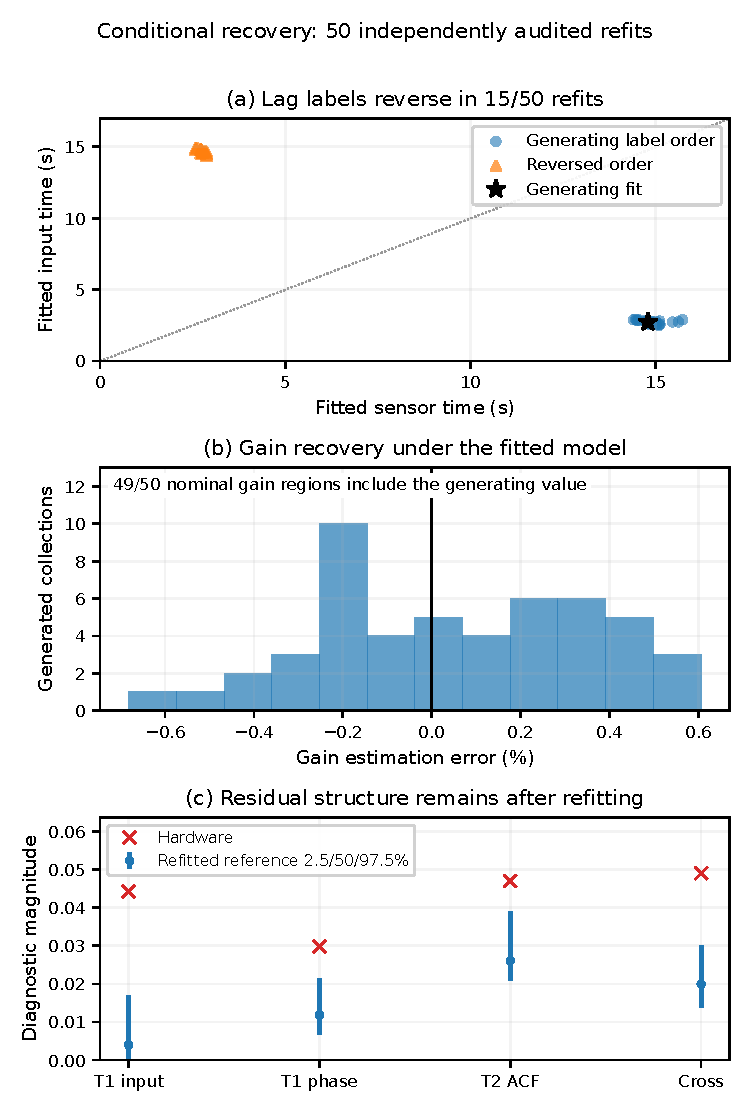
\includegraphics[width=\linewidth]{images/recovery_report.pdf}
\caption{Conditional recovery from fifty fully audited refits. Lag labels
exchange while the two time scales remain separated. The gain calculation
checks nominal scalar LR coverage only. Hardware residual diagnostics exceed
the refitted ranges; the analysis has not resolved their cause.}
\end{figure}

\subsection*{All twenty canonical transfer folds}
Twelve fits omit one run each. Four band-model fits and four shared-conductance
fits omit one protocol each (30, 120 or 300 s sine, or step). Every selected fit
and canonical forecast passed independent audits. No later test temperatures
estimate ambient, conductance or physical parameters; only the first temperature
pair initializes the physical states. Each record appears once per comparison
group, 10,795 scored readings per channel. Groups reuse these same observations;
all records informed structure selection, so transfer is retrospective.

\begin{tabularx}{\linewidth}{@{}Xrr@{}}
\toprule
Nominal reported-mean RMSE, $\C$ & T1 & T2\\
\midrule
Band: omit one run & 1.750 & 0.754\\
Band: omit protocol & 2.131 & 0.875\\
Shared: omit protocol & 2.171 & 0.894\\
\bottomrule
\end{tabularx}

Allowing conductance variation improves the all-data fit much more than these
nominal protocol predictions. Other repeats in training help the leave-run
case. Run mean errors account for 84.9/72.5\% of its T1/T2 SSE; removing them
leaves RMSE $0.680/0.395\C$. For omitted protocols, the band model gives
85.7/73.2\% and $0.806/0.453\C$. Offset removal uses the test outcomes and
cannot serve as a blind correction.

\begin{tabularx}{\linewidth}{@{}Xrr@{}}
\toprule
Range and group & Coverage, \% & Mean width, $\C$\\
 & T1/T2 & T1/T2\\
\midrule
Band/run, noise & 46.01/47.56 & 2.093/0.291\\
Band/run, conditions + noise & 100.00/99.94 & 9.160/5.170\\
Band/protocol, noise & 32.07/36.66 & 2.010/0.303\\
Band/protocol, conditions + noise & 99.57/99.95 & 9.072/5.173\\
Shared/protocol, noise & 50.25/53.46 & 3.606/0.811\\
Shared/protocol, conditions + noise & 94.01/99.81 & 6.769/3.969\\
\bottomrule
\end{tabularx}

Nominal conditions set the unknown run's conductance ratio to one and ambient
offset to zero. Condition ranges allow $\pm2\C$ ambient and, for the band
model, $\pm10\%$ conductance. They combine hard scenario limits with marginal
noise quantiles. Higher coverage accompanies broad ranges; neither candidate
has established calibrated total-95\% predictions or an environmental cause.
The shared model's larger residual variance gives broader noise-only ranges.
Correlated readings do not become independent validation replicates.

The first complete parameter propagation check omits the three fast-sine runs.
Its audited, box-truncated local normal fixes the selected active loading bound
and conditions on one likelihood basin. Adding 256 draws changes condition-plus-noise
mean widths from $9.119/5.134\C$ to $9.223/5.206\C$.
Using 256 instead of the shared-prefix 64 draws moves 2.26/2.69\% of endpoints,
by at most one reported code (0.33 C). This checks mixture resolution, not
coverage calibration or released-bound/basin uncertainty. Four full
components are audited; sixteen remain, including two stopped information
gates under investigation. The local joint-bin log-input-lag SE
without fast-sine data is 0.1232, versus 0.0324 in the twelve-run fit.

Each retained subset also defines a different geometric nominal conductance.
Compare invariant combinations $K_0/t_A=\beta/C_H$, $r/t_A=U_s/C_H$ and
$q/t_A=U_x/C_H$ before treating shifts in $K_0$ as physical change. Centering
a hypothetical twelve-run cohort with the same hard band permits an omitted
run's ratio to a nine-run training nominal in $[0.86894,1.13551]$.
A source-bound arithmetic check verifies these limits and unchanged canonical
forecasts. A separately declared forecast stress check will propagate this
range while preserving the training fits. It is not a transported cohort
likelihood or a corrected coverage calibration.

The refitted checks retain input-linked residual structure. Remaining
questions include whether the conductance band transfers
across protocols, how startup/threshold assumptions assign the lag labels,
and which uncertainty statements survive refitting and simulation.
A future hood experiment should log ambient temperature, absolute time, prior
run recovery, airflow settings, firmware and electrical power. A hood can add
forced or fluctuating convection; it does not automatically supply a constant
environment. No new hardware or DoE is part of this study.

\section*{Evidence and status}
This draft uses terminal, independently audited intermediate artifacts in
the committed remaining-error study. The full decision-gate audit, final
figures and parameter-inclusive uncertainty/transfer results are pending.
It will be replaced after those gates are assessed.

\begin{thebibliography}{9}
\bibitem{park2020}
Park, Martin, Kelly and Hedengren (2020).
Benchmark temperature microcontroller for process dynamics and control.
\emph{Computers \& Chemical Engineering}, article 106736.
\url{https://doi.org/10.1016/j.compchemeng.2020.106736}.
\bibitem{poyiadjis2011}
Poyiadjis, Doucet and Singh (2011).
Particle approximations of the score and observed information matrix in
state space models with application to parameter estimation.
\emph{Biometrika}, 98, 65--80.
\url{https://www.stats.ox.ac.uk/~doucet/poyiadjis_doucet_singh_particlescoreparameterestimation.pdf}.
\bibitem{dunn1996}
Dunn and Smyth (1996). Randomized quantile residuals.
\emph{Journal of Computational and Graphical Statistics}, 5, 236--244.
\url{https://gksmyth.github.io/pubs/residual.pdf}.
\end{thebibliography}
\end{document}
